Skemalægningsprogrammet Docendo er et brugervenligt samt forholdsvis simpelt program. Programmet går ud på, at der dannes en kalender med uger og dage, hvorefter brugeren har mulighed for at justere diverse parametre alt efter behov. Heriblandt tager programmet bl.a. højde for, at nogle skoler har forskellige fag, og giver derfor brugeren mulighed for at tilføje et eller flere fag. Samtidig har brugeren mulighed for at tilpasse lektionernes længde, hvilket også er en essentiel parameter, da nogle skoler forsøger på at undgå tunge fag om eftermiddagen eksempelvis. Dernæst fastlåser programmet lokaler og lærere som har undervisning på bestemte tidspunkter, så brugeren fortsat har overblik over skemaplanlægningen og så der ikke opstår dobbeltbookninger af et bestemt lokale eller lignende. Hvis et problem skulle opstå, kan lektionerne flyttes med et simpelt klik, og de nye skemaer bliver genereret i ét, hvilket igen gør at der er fortsat overblik over skemalægningen\cite{docendo}.
\begin{figure}[!h]
  \centering
  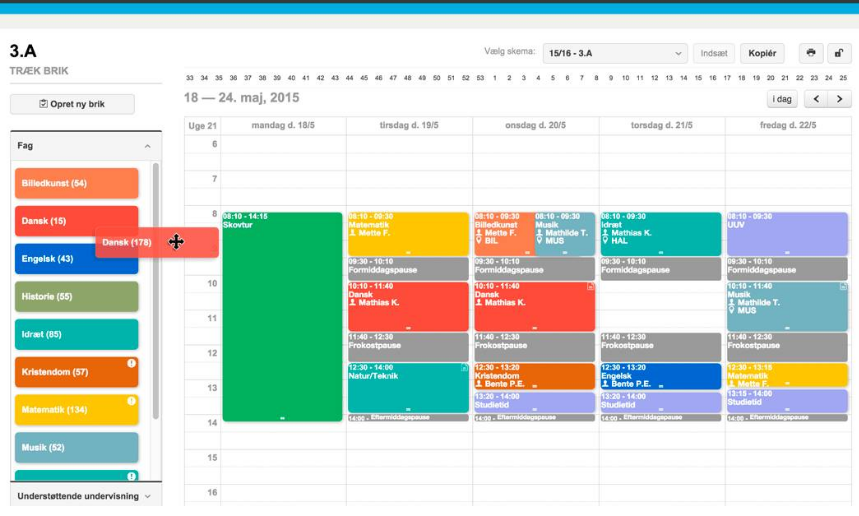
\includegraphics[width=\textwidth]{partials/graphics/docendo.png}
    \caption{Eksempel på skemplanlægning i Docendo\cite{docendob}.}
  \label{fig:docendo}
\end{figure}

